\ifx\wholebook\relax\else
\documentclass[twoside]{book}
\usepackage[active]{srcltx}
\usepackage[LY1]{fontenc}
\usepackage{epsfig}
\def\etc{{\it etc}}
\def\eg{{\it e.g.}}
\def\ie{{\it i.e.}}
\def\cf{{\it c.f.}\ }
\def\erf{\mathop{\rm erf}}
\def\sign{\mathop{\rm sign}}
\def\prob{\mathop{\rm Prob}}
\def\var{\mathop{\rm var}}
\def\mod{\mathop{\rm mod}}
\def\cor{\mathop{\rm cor}}
\def\cov{\mathop{\rm cov}}
\def\cl{\mathop{\rm CL}}
\def\kg{\mathop{\rm Kg}}
\def\patstyle#1{{\sc #1}}
\def\th{^{\mathop{\rm th}}}
\def\st#1{^{\mathop{\rm #1}}}
\def\note#1{\begin{quote}{\bf Note:} #1\end{quote}}
\def\braket#1{\left\langle #1\right\rangle}
\def\order#1{\let\o=#1{\cal O}\ifx\o 1$\left(n\right)$\else$\left(n^{#1}\right)$\fi}
\newtheorem{privListing}{Listing}[chapter]
\newenvironment{listing}{\vskip 3ex\hrule\vskip 1ex\begin{privListing}}{\end{privListing}\hrule\vskip 1ex}
\newtheorem{privExample}{Code example}[chapter]
\newenvironment{codeExample}{\begin{privExample}\begin{quote}\tt}{\end{quote}\end{privExample}}
\def\relboxl#1#2{\hbox to #1\hsize{#2\hfil}}
\def\relboxc#1#2{\hbox to #1\hsize{\hfil #2\hfil}}
\def\relboxr#1#2{\hbox to #1\hsize{\hfil #2}}
\def\transpose#1{{\bf #1}^{\mathop{\rm T}}}
\def\inverse#1{{\bf #1}^{-1}}
%\def\tm{$^{\mathop{\rm TM}}$}
\def\tm{ }
\newenvironment{mainEquation}{\marginpar[\vspace{3 ex} Main
equation$\Rightarrow$]{\vspace{3 ex}$\Leftarrow$Main
equation}\begin{equation}}{\end{equation}}
\def\rubrique#1{\paragraph{#1}\hfil\par\noindent}

\begin{document}
\fi

\chapter{Data mining} \vspace{1 ex}
\begin{flushright} {\sl Creusez, fouillez, b\^echez, ne laissez nulle place}\\
{\sl O\`{u} la main ne passe et repasse,}\footnote{Dig, search,
excavate, do not leave a place where your hands did not go once or
more.}\\ Jean de La Fontaine
\end{flushright}
\vspace{1 ex} \label{ch:datamining} Data mining is a catchy
buzz-word of recent introduction covering activities formerly
known as data analysis. The problem is akin to what we already
have seen in chapter \ref{ch:estimation}. In the case of data
mining, however, the emphasis is put on large data sets. {\sl
Large} must be understood in to ways: first, each {\sl data point}
is actually made of a large number of measurements; second, the
number of data points is large, even huge. The expression data
mining was coined when large corporate databases become common
place. The original reason for the presence of these databases was
the day to day dealing with the business events. A few people
started realizing that these databases are containing huge amount
of information, mostly of statistical nature, about the type of
business. That information was just waiting to be mined just like
the Mother Lode waited for the coming of the 49ers. Hence the term
data mining.

Figure \ref{fig:dataminingclasses} shows the classes described in
this chapter.
\begin{figure}
\centering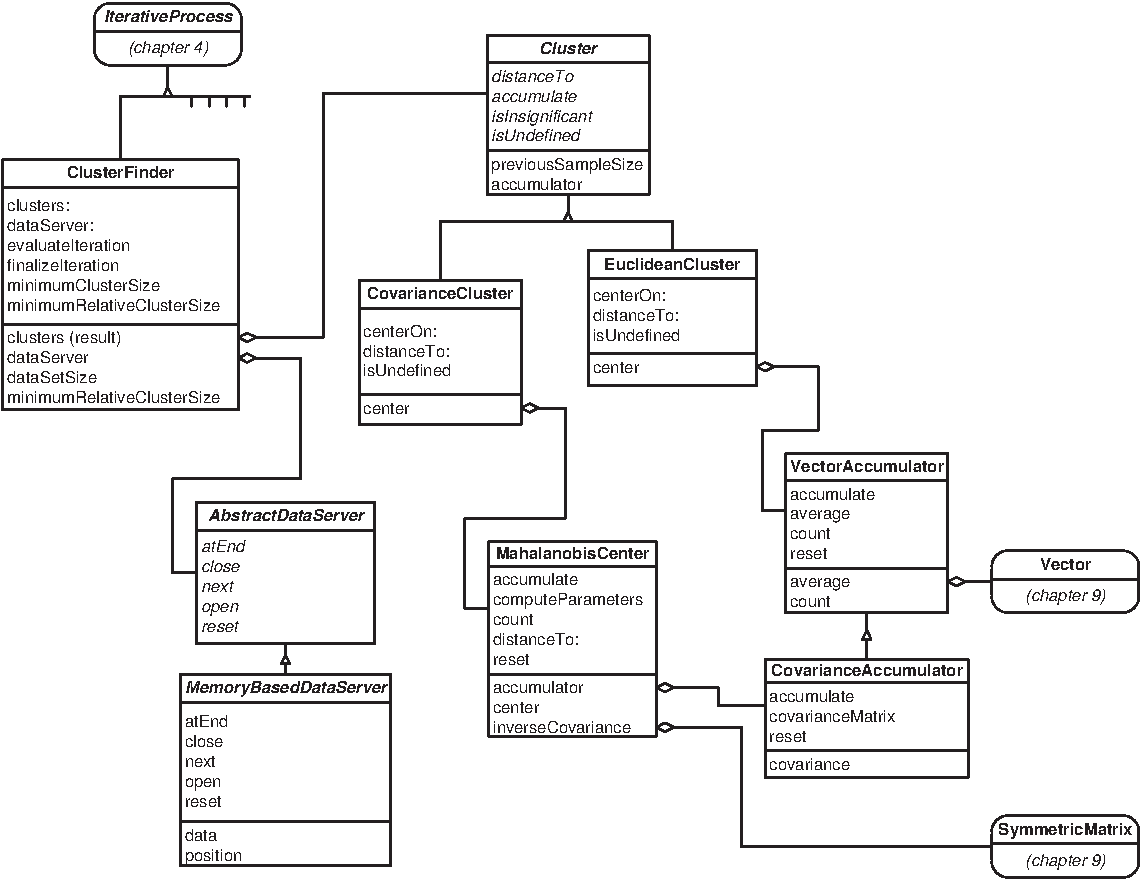
\includegraphics[width=11cm]{Figures/DataminingClasses}
\caption{Classes used in data mining}\label{fig:dataminingclasses}
\end{figure}
There are two aspects to the data mining activity: one is
preparing the data in order to render them suitable for the
processing; the second consists of extracting the information,
that is, the processing of the data. Depending on the problems and
on the technique used during the second step , the first step is
not always needed. In any case, the preparation of the data is
usually very specific to the type of data to be analyzed.
Therefore one can only make very general statements about this
problem: one must watch for rounding errors; one must adjust the
scale of data having widely different ranges; one must check the
statistical validity of the data sample; \etc. We shall say no
more about this first aspect of data mining, but we wanted to warn
the reader about this important issue.

Finally, data mining differs from estimation in that, in many
cases the type of information to be extracted is not really known
in advance. Data mining tries to identify trends, common
properties and correlation between the data. The goal of data
mining is usually to reduce large sample to much smaller
manageable sets, which can be efficiently targeted. One example,
is the selection of a sample of customers suitable to respond to a
new product offered by a bank or an insurance company. Mailing
operations are costly; thus, any reduction of the mailing target
set with a significant improvement of the probability of response
can bring a significant saving. Another example in the medical
domain is the scanning for certain type of cancer, which are
expensive\footnote{In medical domain, {\sl expensive} is not
necessarily a matter of money. It can mean high risk for the
patient or the examination is regarded as too intrusive by the
patient.}. If one can identify a population with high risk of
cancer, the scanning only needs to done for that population, thus
keeping the cost low.

A good collection of articles about the techniques exposed in this
chapter can be found in \cite{AtchBry}.

\section{Data server}
\label{sec:dataserver} \marginpar{Figure
\ref{fig:dataminingclasses} with the boxes {\bf
AbstractDataServer} and {\bf MemoryBasedDataServer} grayed.} As we
have said in the introduction, data mining means handling large
amounts of data, most likely more than the computer memory can
hold. Thus, we need an object to handle these data for all objects
implementing data mining techniques.

\noindent The data server object needs to implement five
functionalities:
\begin{enumerate}
  \item opening the physical support of the data,
  \item getting the next data item,
  \item checking whether more data items are available,
  \item repositioning the data stream at its beginning and
  \item closing the physical support of the data.
\end{enumerate}
Depending on the problem at hand, the responsibility of a data
server can extend beyond the simple task of handling data. In
particular, it could be charged of performing the data preparation
step mentioned in the introduction. In our implementation, we give
two classes. One is an abstract class from which all data servers
used by the data mining objects described in this chapter must
derive. The data item returned by the method returning the nest
item is a vector object whose components are the data
corresponding to one measurement. The second class of data server
is a concrete class implementing the data server on a collection
or array kept in the computer's memory. Such server is handy for
making tests.

\note{Examples of use of data server are given in the other
sections; no code example are given here.}

\subsection{Data server --- Smalltalk implementation}
\label{sec:sdataserver} Listing \ref{ls:abstractserver} shows the
implementation of the abstract data server in Smalltalk. The
implementation of the concrete class is shown in listing
\ref{ls:memoryserver}.

\noindent Our implementation uses the same methods used by the
hierarchy of the class {\tt Stream}.

\begin{listing} Smalltalk abstract data server \label{ls:abstractserver}
$$\halign{ #\hfil&\quad#\hfil\cr {\sl Class}& {\Large\bf DhbAbstractDataServer}\cr
{\sl Subclass of }&{\tt Object}\cr\noalign{\vskip 1ex}
}$$


Instance methods
{\parskip 1ex\par\noindent}
{\bf atEnd}
\begin{verbatim}
    self subclassResponsibility

\end{verbatim}
{\bf close}
\begin{verbatim}

\end{verbatim}
{\bf next}
\begin{verbatim}
    self subclassResponsibility

\end{verbatim}
{\bf open}
\begin{verbatim}
    self subclassResponsibility

\end{verbatim}
{\bf reset}
\begin{verbatim}
    self subclassResponsibility

\end{verbatim}


\end{listing}
\begin{listing} Smalltalk memory based data server \label{ls:memoryserver}
$$\halign{ #\hfil&\quad#\hfil\cr {\sl Class}& {\Large\bf DhbMemoryBasedDataServer}\cr
{\sl Subclass of }&{\tt DhbAbstractDataServer}\cr\noalign{\vskip 1ex}

{\sl Instance variable names:}&\parbox[t]{4 in}{\tt  data position }\cr\noalign{\vskip 1ex}}$$


Instance methods
{\parskip 1ex\par\noindent}
{\bf atEnd}
\begin{verbatim}
    ^ data size < position
\end{verbatim}
{\bf data:} {\tt anOrderedCollection}
\begin{verbatim}
    data := anOrderedCollection.
    self reset.
\end{verbatim}
{\bf dimension}
\begin{verbatim}
    ^ data first size
\end{verbatim}
{\bf next}
\begin{verbatim}
    | answer |
    answer := data at: position.
    position := position + 1.
    ^ answer
\end{verbatim}
{\bf open}
\begin{verbatim}
    self reset
\end{verbatim}
{\bf reset}
\begin{verbatim}
    position := 1.
\end{verbatim}


\end{listing}

\section{Covariance and covariance matrix}
\label{sec:covmatrix} When one deals with two or more random
variables an important question to ask is whether or not the two
variables are dependent from each other.

For example, if one collects the prices of homes and the incomes
of the home owners,one will find that inexpensive homes are mostly
owned by low income families, {\sl mostly but not always}. It is
said that the price of a home is {\sl correlated} with the income
of the home owner. As soon as one deals with more than two
variables things stop being clear cut. Correlations become hard to
identify especially because of these {\sl mostly but not always}
cases. Therefore, one must find a way to expressed mathematically
how much two random variables are correlated.

Let $x_1,\ldots,x_m$ be several random variable. They can be
considered as the components of a $m$-dimensional(random) vector
${\bf x}$. The probability density function of the vector ${\bf
x}$ is denoted $P\left({\bf x}\right)$; it measures the
probability of observing a vector within the differential volume
element located at ${\bf x}$. The average of the vector ${\bf x}$
is defined in a way similar to the case of a single random
variable. The $i\th$ component of the average is defined by
\begin{equation}
 \mu_i=\int\ldots\int x_i P\left({\bf x}\right)dx_1\ldots dx_m.
\end{equation}
The covariance matrix of the random vector ${\bf x}$ gives a
measure of the correlations between the components of the vector
${\bf x}$. The components of the covariance matrix are defined by
\begin{equation}
 \varrho_{ij}=\int\ldots\int \left(x_i-\mu_i\right)\left(x_j-\mu_j\right)
  P\left({\bf x}\right)dx_1\ldots dx_m.
\end{equation}
As one can see the covariance matrix is a symmetric matrix. It is
also positive definite. Furthermore $\varrho_{ii}$ is the variance
of the $i\th$ component of the random vector.

 \note{The error matrix of a least square or maximum
likelihood fit --- discussed in chapter \ref{ch:estimation} --- is
the covariance matrix of the fit parameters.}

If two components are independent, their covariance --- that is,
the corresponding element of the covariance matrix --- is zero.
The inverse is not true, however. For example, consider a
2-dimensional vector with components $\left(z z^2\right)$ where
$z$ is a random variable. If $z$ is distributed according to a
symmetric distribution, the covariance between the two components
of the vector is zero. Yet, the components are $100\%$ dependent
from each other by construction.

The correlation coefficient between components $i$ and $j$ of the
vector ${\bf x}$ is then defined by
\begin{equation}
 \rho_{ij}={\varrho_{ij}\over \sigma_i \sigma_j},
\end{equation}
where $\sigma_i=\sqrt{\varrho_{ii}}$ is the standard deviation of
the $i\th$ component of the vector ${\bf x}$. By definition, the
correlation coefficient is comprised between $-1$ and $1$. If the
absolute value of a correlation coefficient is close to $1$ then
one can assert that the two corresponding components are indeed
correlated.

If the random vector is determined experimentally, one calculates
the estimated covariance with the following statistics
\begin{equation}
 \cov\left(x_i,x_j\right)={1\over n}\sum_{k=1}^n
 \left(x_{i,k}-\mu_i\right)\left(x_{j,k}-\mu_j\right),
\end{equation}
where $x_{i,k}$ is the $i\th$ component of the $k\th$ measurement
of the vector ${\bf x}$. Similarly the estimated correlation
coefficient of the corresponding components is defined as
\begin{equation}
 \cor\left(x_i,x_j\right)={\cov\left(x_i,x_j\right)\over s_i s_j},
\end{equation}
where $s_i$ is the estimated standard deviation of the $i\th$
component.

Like for the central moment, there is a way to compute the
components of the covariance matrix while they are accumulated. If
${\cov}_n\left(x_i,x_j\right)$ denotes the estimated covariance
over $n$ measurements, one has:
\begin{equation}
\label{eq:robustcov}
 {\cov}_{n+1}\left(x_i,x_j\right)={n\over
 n+1}{\cov}_n\left(x_i,x_j\right)+n\Delta_{i,n+1}\Delta_{j,n+1},
\end{equation}
where $\Delta_{x,n+1}$ and $\Delta_{y,n+1}$ are the corrections to
the averages of each variable defined in equation
\ref{eq:deltaverage} of section \ref{sec:robustmoment}. The
derivation of equation \ref{eq:robustcov} is given in appendix
\ref{sec:robustcov}.

\rubrique{Using covariance information} A covariance matrix
contains statistical information about the set of measurements
over which is has been determined. There are several ways of using
this information.

The first approach uses the covariance matrix directly. The best
example is the analysis known as the shopping cart analysis
\cite{BerLin}. For example, one can observe that consumers buying
cereals are buying low fat milk. This can give useful information
on how to target special sales efficiently. Application working in
this mode can use the code of sections \ref{sec:scovmatrix} or
\ref{sec:jcovmatrix} as is.

Another approach is to use the statistical information contained
in a covariance matrix to process data coming from measurements
which were not used to determine the covariance matrix. In the
rest of this chapter we shall call the set of measurements, which
is used to determine the covariance matrix, the {\sl calibrating
set}. In this second mode of using a covariance matrix,
measurements are {\sl compared} or {\sl evaluated} against those
of the calibrating set. It is clear that the quality of the
information contained in the covariance matrix depends on the
quality of the calibrating set. We shall assume that this is
always the case. Techniques working according to this second mode
are described in sections \ref{sec:datared}, \ref{sec:mahalanobis}
and \ref{sec:mahalanobiscluster}.

\subsection{Covariance matrix --- General implementation}
\marginpar{Figure \ref{fig:dataminingclasses} with the boxes {\bf
VectorAccumulator} and {\bf CovarianceAccumulator} grayed.} The
object in charge of computing the covariance matrix of a series of
measurements is implemented as for central moments. Because we
shall need to only compute the average of a vector, the
implementation is spread over two classes, one being the subclass
of the other for efficient reuse.

\noindent The class {\tt VectorAccumulator} has two instance
variables: {} {\parskip 0pt
\begin{description}
  \item[\tt count] counts the number of vectors accumulated in the object so far;
  \item[\tt average] keeps the average of the accumulated vector;
\end{description}
}

\noindent The class {\tt CovarianceAccumulator} is a subclass of
the class {\tt VectorAccumulator}. It has one additional instance
variable: {} {\parskip 0pt
\begin{description}
  \item[\tt covariance] accumulates the components of the covariance
  matrix; for efficiency reason, only the lower half of the matrix
  is computed since it is symmetric.
\end{description}
}

The topmost class implements equation \ref{eq:deltaverage} in the
method {\tt accumulate}. The subclass overloads this method to
implement equation \ref{eq:robustcov}.

\subsection{Covariance matrix --- Smalltalk implementation}
\label{sec:scovmatrix} Listing \ref{ls:vectoraverage} shows the
implementation of the accumulation of a vector in Smalltalk.
Listing \ref{ls:covmatrix} shows the implementation of the
accumulation of the covariance matrix. The following code example
shows how to accumulate the average of a series of vectors read
from a data stream.
\begin{codeExample}
\begin{verbatim}

 | accumulator valueStream average |
 accumulator := DhbVectorAccumulator new.
 valueStream open.
 [ valueStream atEnd ]
        whileFalse: [ accumulator accumulate: valueStream next ].
 valueStream close.
 average := accumulator average.
\end{verbatim}
\end{codeExample}
The reader can see that this example is totally equivalent to the
code example \ref{ex:smoments}. Here the method {\tt next} of the
data stream must return a vector instead of a number; all vectors
must have the same dimension. The returned average is a vector of
the same dimension.

The next code example shows how to accumulate the both average and
covariance matrix. The little differences with the preceding
example should be self explanatory to the reader.
\begin{codeExample}
\begin{verbatim}

 | accumulator valueStream average covarianceMatrix |
 accumulator := DhbCovarianceAccumulator new.
 valueStream open.
 [ valueStream atEnd ]
        whileFalse:[ accumulator accumulate: valueStream next ].
 valueStream close.
 average := accumulator average.
 covarianceMatrix := accumulator covarianceMatrix.
\end{verbatim}
\end{codeExample}

The method {\tt accumulate} of class {\tt DhbVectorAccumulator}
answers the corrections to each component of the average vector.
This allows the class {\tt DhbCovarianceAccumulator} to reuse the
results of this method. In class {\tt DhbVectorAccumulator},
vector operations are used. The method {\tt accumulate} of class
{\tt DhbCovarianceAccumulator} works with indices because one only
computes the lower half of the matrix.

\begin{listing} Smalltalk implementation of vector average \label{ls:vectoraverage}
$$\halign{ #\hfil&\quad#\hfil\cr {\sl Class}& {\Large\bf DhbVectorAccumulator}\cr
{\sl Subclass of }&{\tt Object}\cr\noalign{\vskip 1ex}

{\sl Instance variable names:}&\parbox[t]{4 in}{\tt  count average }\cr\noalign{\vskip 1ex}}$$


Class methods
{\parskip 1ex\par\noindent}
{\bf new:} {\tt anInteger}
\begin{verbatim}
    ^self new initialize: anInteger

\end{verbatim}



Instance methods
{\parskip 1ex\par\noindent}
{\bf accumulate:} {\tt aVectorOrArray}
\begin{verbatim}
    | delta |
    count := count + 1.
    delta := average - aVectorOrArray asVector scaleBy: 1 / count.
    average accumulateNegated: delta.
    ^delta

\end{verbatim}
{\bf average}
\begin{verbatim}
    ^average

\end{verbatim}
{\bf count}
\begin{verbatim}
    ^count

\end{verbatim}
{\bf initialize:} {\tt anInteger}
\begin{verbatim}
    average := DhbVector new: anInteger.
    self reset.
    ^self

\end{verbatim}
{\bf printOn:} {\tt aStream}
\begin{verbatim}
    super printOn: aStream.
    aStream space.
    count printOn: aStream.
    aStream space.
    average printOn: aStream.   

\end{verbatim}
{\bf reset}
\begin{verbatim}
    count := 0.
    average atAllPut: 0.

\end{verbatim}


\end{listing}

\begin{listing} Smalltalk implementation of covariance matrix \label{ls:covmatrix}
$$\halign{ #\hfil&\quad#\hfil\cr {\sl Class}& {\Large\bf DhbCovarianceAccumulator}\cr
{\sl Subclass of }&{\tt DhbVectorAccumulator}\cr\noalign{\vskip 1ex}

{\sl Instance variable names:}&\parbox[t]{4 in}{\tt  covariance }\cr\noalign{\vskip 1ex}}$$


Instance methods
{\parskip 1ex\par\noindent}
{\bf accumulate:} {\tt anArray}
\begin{verbatim}
    | delta count1 r|
    count1 := count.
    delta := super accumulate: anArray.
    r := count1 / count.
    1 to: delta size
        do: [ :n |
              1 to: n do:
                  [ :m |
                    ( covariance at: n) at: m put: ( count1 * ( delta 
       at: n) * ( delta at: m) + ( r * ( ( covariance at: n) at: m))).
                  ].
            ].

\end{verbatim}
{\bf covarianceMatrix}
\begin{verbatim}
    | rows n |
    n := 0.
    rows := covariance collect:
                [ :row | n := n + 1. row, ( ( ( n + 1) to: covariance 
                  size) collect: [ :m | ( covariance at: m) at: n ])].
    ^DhbSymmetricMatrix rows: rows

\end{verbatim}
{\bf initialize:} {\tt anInteger}
\begin{verbatim}
    covariance := ( ( 1 to: anInteger) collect: [ :n | DhbVector new: 
                                                         n]) asVector.
    ^super initialize: anInteger

\end{verbatim}
{\bf reset}
\begin{verbatim}
    super reset.
    covariance do: [ :each | each atAllPut: 0].

\end{verbatim}


\end{listing}



\section{Multidimensional probability distribution}
\label{sec:multiprob} To get a feeling of what the covariance
matrix represents, let us now consider a vector ${\bf y}$ whose
components are independent random variables distributed according
to a normal distribution. The probability density function is
given by
\begin{equation}
\label{eq:multiprob} P\left({\bf y}\right) = \prod_{i=1}^m{
1\over\sqrt{2\pi\sigma_i^2}}e^{-{\left(y_i-\mu_i\right)^2\over
2\sigma_i^2}}.
\end{equation}
In this case, the covariance matrix of the vector ${\bf y}$ is a
diagonal matrix $\tilde{\bf{V}}$, whose diagonal elements are the
variance of the vector's components. If $\tilde{\bf{C}}$ is the
inverse of the matrix $\tilde{\bf{V}}$, equation
\ref{eq:multiprob} can be rewritten as
\begin{equation}
P\left({\bf y}\right) =
\sqrt{{\det{\tilde{\bf{C}}}\over\left(2\pi\right)^m}}e^{-{1\over
2}\left({\bf y}-\bar{{\bf y}}\right)^{\mathop{\rm T}}
\tilde{\bf{C}}\left({\bf y}-\bar{{\bf y}}\right)},
\end{equation}
where $\bar{{\bf y}}$ is the vector whose components are
$\mu_1,\ldots,\mu_m$. Let us now consider a change of coordinates
${\bf x}={\bf O}{\bf y}$, where ${\bf O}$ is an orthogonal matrix.
We have already met such transformations in section
\ref{sec:eigensym}. Because the matrix is orthogonal, the
differential volume element is invariant under the change of
coordinates. Thus, the probability density function of the vector
${\bf x}$ is
\begin{equation}
\label{eq:multinorm} P\left({\bf x}\right) =
\sqrt{{\det{\bf{C}}\over\left(2\pi\right)^m}}e^{-{1\over
2}\left({\bf x}-\bar{{\bf x}}\right)^{\mathop{\rm T}}
\bf{C}\left({\bf x}-\bar{{\bf x}}\right)},
\end{equation}
where the matrix ${\bf C}$ is equal to $\transpose{O}\tilde{{\bf
C}}{\bf O}$. The vector $\bar{{\bf x}}$ is simply\footnote{All
this is a consequence of the linear property of the expectation
value operator.} equal to ${\bf O}\bar{{\bf y}}$. The covariance
matrix, ${\bf V}$, of the vector ${\bf x}$ is then equal to
$\transpose{O}\tilde{{\bf V}}{\bf O}$. It is also the inverse of
the matrix ${\bf C}$. Thus, equation \ref{eq:multinorm} can be
rewritten as
\begin{equation}
\label{eq:multinormal} P\left({\bf x}\right) = {1
\over\sqrt{\left(2\pi\right)^m{\det{\bf V}}}}e^{-{1\over
2}\left({\bf x}-\bar{{\bf x}}\right)^{\mathop{\rm T}}
\inverse{V}\left({\bf x}-\bar{{\bf x}}\right)}.
\end{equation}
In the case of a normal distribution in a multi-dimensional space,
the covariance matrix plays the same role as the variance in one
dimension.

\section{Covariance data reduction}
\label{sec:datared} Reversing the derivation of the preceding
section one can see that the eigenvalues of the covariance matrix
of the vector ${\bf x}$ correspond to the variances of a series of
independent\footnote{Not necessarily normally distributed!} random
variables $y_1,\dots,y_m$. Since the covariance matrix is
symmetric these eigenvalues as well as the matrix ${\bf O}$
describing the change of coordinates can be obtained using
Jacobi's algorithm described in section \ref{sec:eigensym}.

If some eigenvalues are much larger than the others, one can state
that the information brought by the corresponding variables brings
little information to the problem. Thus, one can omit the
corresponding variable from the rest of the analysis.

Let $\sigma^2_1,\ldots,\sigma^2_m$ be the eigenvalues of the
covariance matrix such that $\sigma^2_i < \sigma^2_j$ for $i<j$.
Let us assume that there exist an index $k$ such that $\sigma^2_k
\gg \sigma^2_{k-1}$. Then,  The rest of the data analysis can be
made with a vector with components $y_k,\ldots,y_m$ where the
vector ${\bf y}$ is defined by ${\bf y}=\transpose{O}{\bf x}$.

This reduction technique has been used successfully in high energy
physics\footnote{H.Wind, {\em Pattern recognition by principal
component analysis of border regions}, Proceedings $3^{\mathop{\rm
th}}$ topical meeting on multi-dimensional analysis of high energy
data, Nijmegen, 8-11 March 1978, W. Kittel, University of
Nijmegen, 1978, pp. 99-106.} under the name principal component
analysis. The data reduction allows to extract the relevant
parameters of a complex particle detector to facilitate the quick
extraction of the physical data --- momentum and energy of the
particle --- from the observed data.

This kind of data reduction can be implemented within the
framework of the data server described in section
\ref{sec:dataserver}. The concrete implementation of such a server
is straight forward. All needed objects --- covariance
accumulation, eigenvalues of a symmetric matrix, vector
manipulation --- have been discussed in different chapters. The
rest of the implementation is specific to the problem at hand and
can therefore not be treated on a general basis.

\section{Mahalanobis distance}
\label{sec:mahalanobis} Mahalanobis, an Indian statistician,
introduced this distance in the 30's when working on
anthropometric statistics. A paper by Mahalanobis himself can be
found in \cite{AtchBry}. Readers interested by the historical
dimension of the Mahalanobis distance can consult the paper by Das
Gupta\footnote{Somesh Das Gupta, \em{The evolution of the $D\sp
2$-statistics of Mahalanobis}, Indian J. Pure Appl. Math., {\bf
26}(1995), no. 6, 485-501.}.

By definition, the exponent of equation \ref{eq:multiprob} is
distributed according to a $\chi^2$ distribution with $m$ degrees
of freedom. This exponent remains invariant under the change of
coordinates discussed in section \ref{sec:multiprob}. Thus, the
exponent of equation \ref{eq:multinormal} is also distributed
according to a $\chi^2$ distribution with $m$ degrees of freedom,
where $m$ is the dimension of the vector $x$. The Mahalanobis
distance, $d_M$, is defined as the square root of the exponent, up
to a factor $\sqrt{2}$. We have
\begin{equation}
\label{eq:mahalanobis} d^2_M = \left({\bf x}-\bar{{\bf
x}}\right)^{\mathop{\rm T}} \inverse{V}\left({\bf x}-\bar{{\bf
x}}\right).
\end{equation}
The Mahalanobis distance is a distance using the inverse of the
covariance matrix as the metric. It is a distance in the
geometrical sense because the covariance matrix as well as its
inverse are positive definite matrices. The metric defined by the
covariance matrix provides a normalization of the data relative to
their spread.

The Mahalanobis distance --- or its square --- can be used to
measure how {\sl close} an object is from another when these
objects can be characterized by a series of numerical
measurements. Using the Mahalanobis distance is done as follows
\begin{enumerate}
  \item the covariance matrix of the measured quantities, ${\bf V}$, is
determined over a calibrating set;
  \item one compute the inverse of the covariance matrix,
  $\inverse{V}$;
  \item the distance of a new object to the calibrating set is
  estimated using equation \ref{eq:mahalanobis}; if the distance
  is smaller than a given threshold value, the new object is
  considered as belonging to the same
\end{enumerate}
One interesting property of the Mahalanobis distance is that it is
normalized. Thus, it is not necessary to normalize the data
provided rounding errors in inverting the covariance matrix are
kept under control. If the data are roughly distributed according
to a normal distribution the threshold for accepting whether or
not an object belongs to the calibrating set can be determined
from the $\chi^2$ distribution.

\rubrique{Examples of use} \noindent The Mahalanobis distance can
be applied in all problems where measurements must be classified.

A good example is the detection of coins in a vending machine.
When a coin is inserted into the machine, a series of sensors
gives several measurements, between a handful and a dozen. The
detector can be calibrated using a set of good coins forming a
calibration set. The coin detector can differentiate good coins
from the fake coins using the Mahalanobis distance computed on the
covariance matrix of the calibration set. Figure
\ref{fig:mahalanobis} shows an example of such data\footnote{Data
are reproduced with permission; the owner of the data wants to
remain anonymous, however.}. The light gray histogram is the
distribution of the Mahalanobis distance of the good coins; the
dark gray histogram that of the fake coins. The dotted line is the
$\chi^2$-distribution corresponding to the degrees of freedom of
the problem; in other words, the distribution was not fitted. The
reader can see that the curve of the $\chi^2$-distribution
reproduces the distribution of the experimental data. Figure
\ref{fig:mahalanobis} also shows the power of separation achieved
between good and fake coins.
\begin{figure}
\centering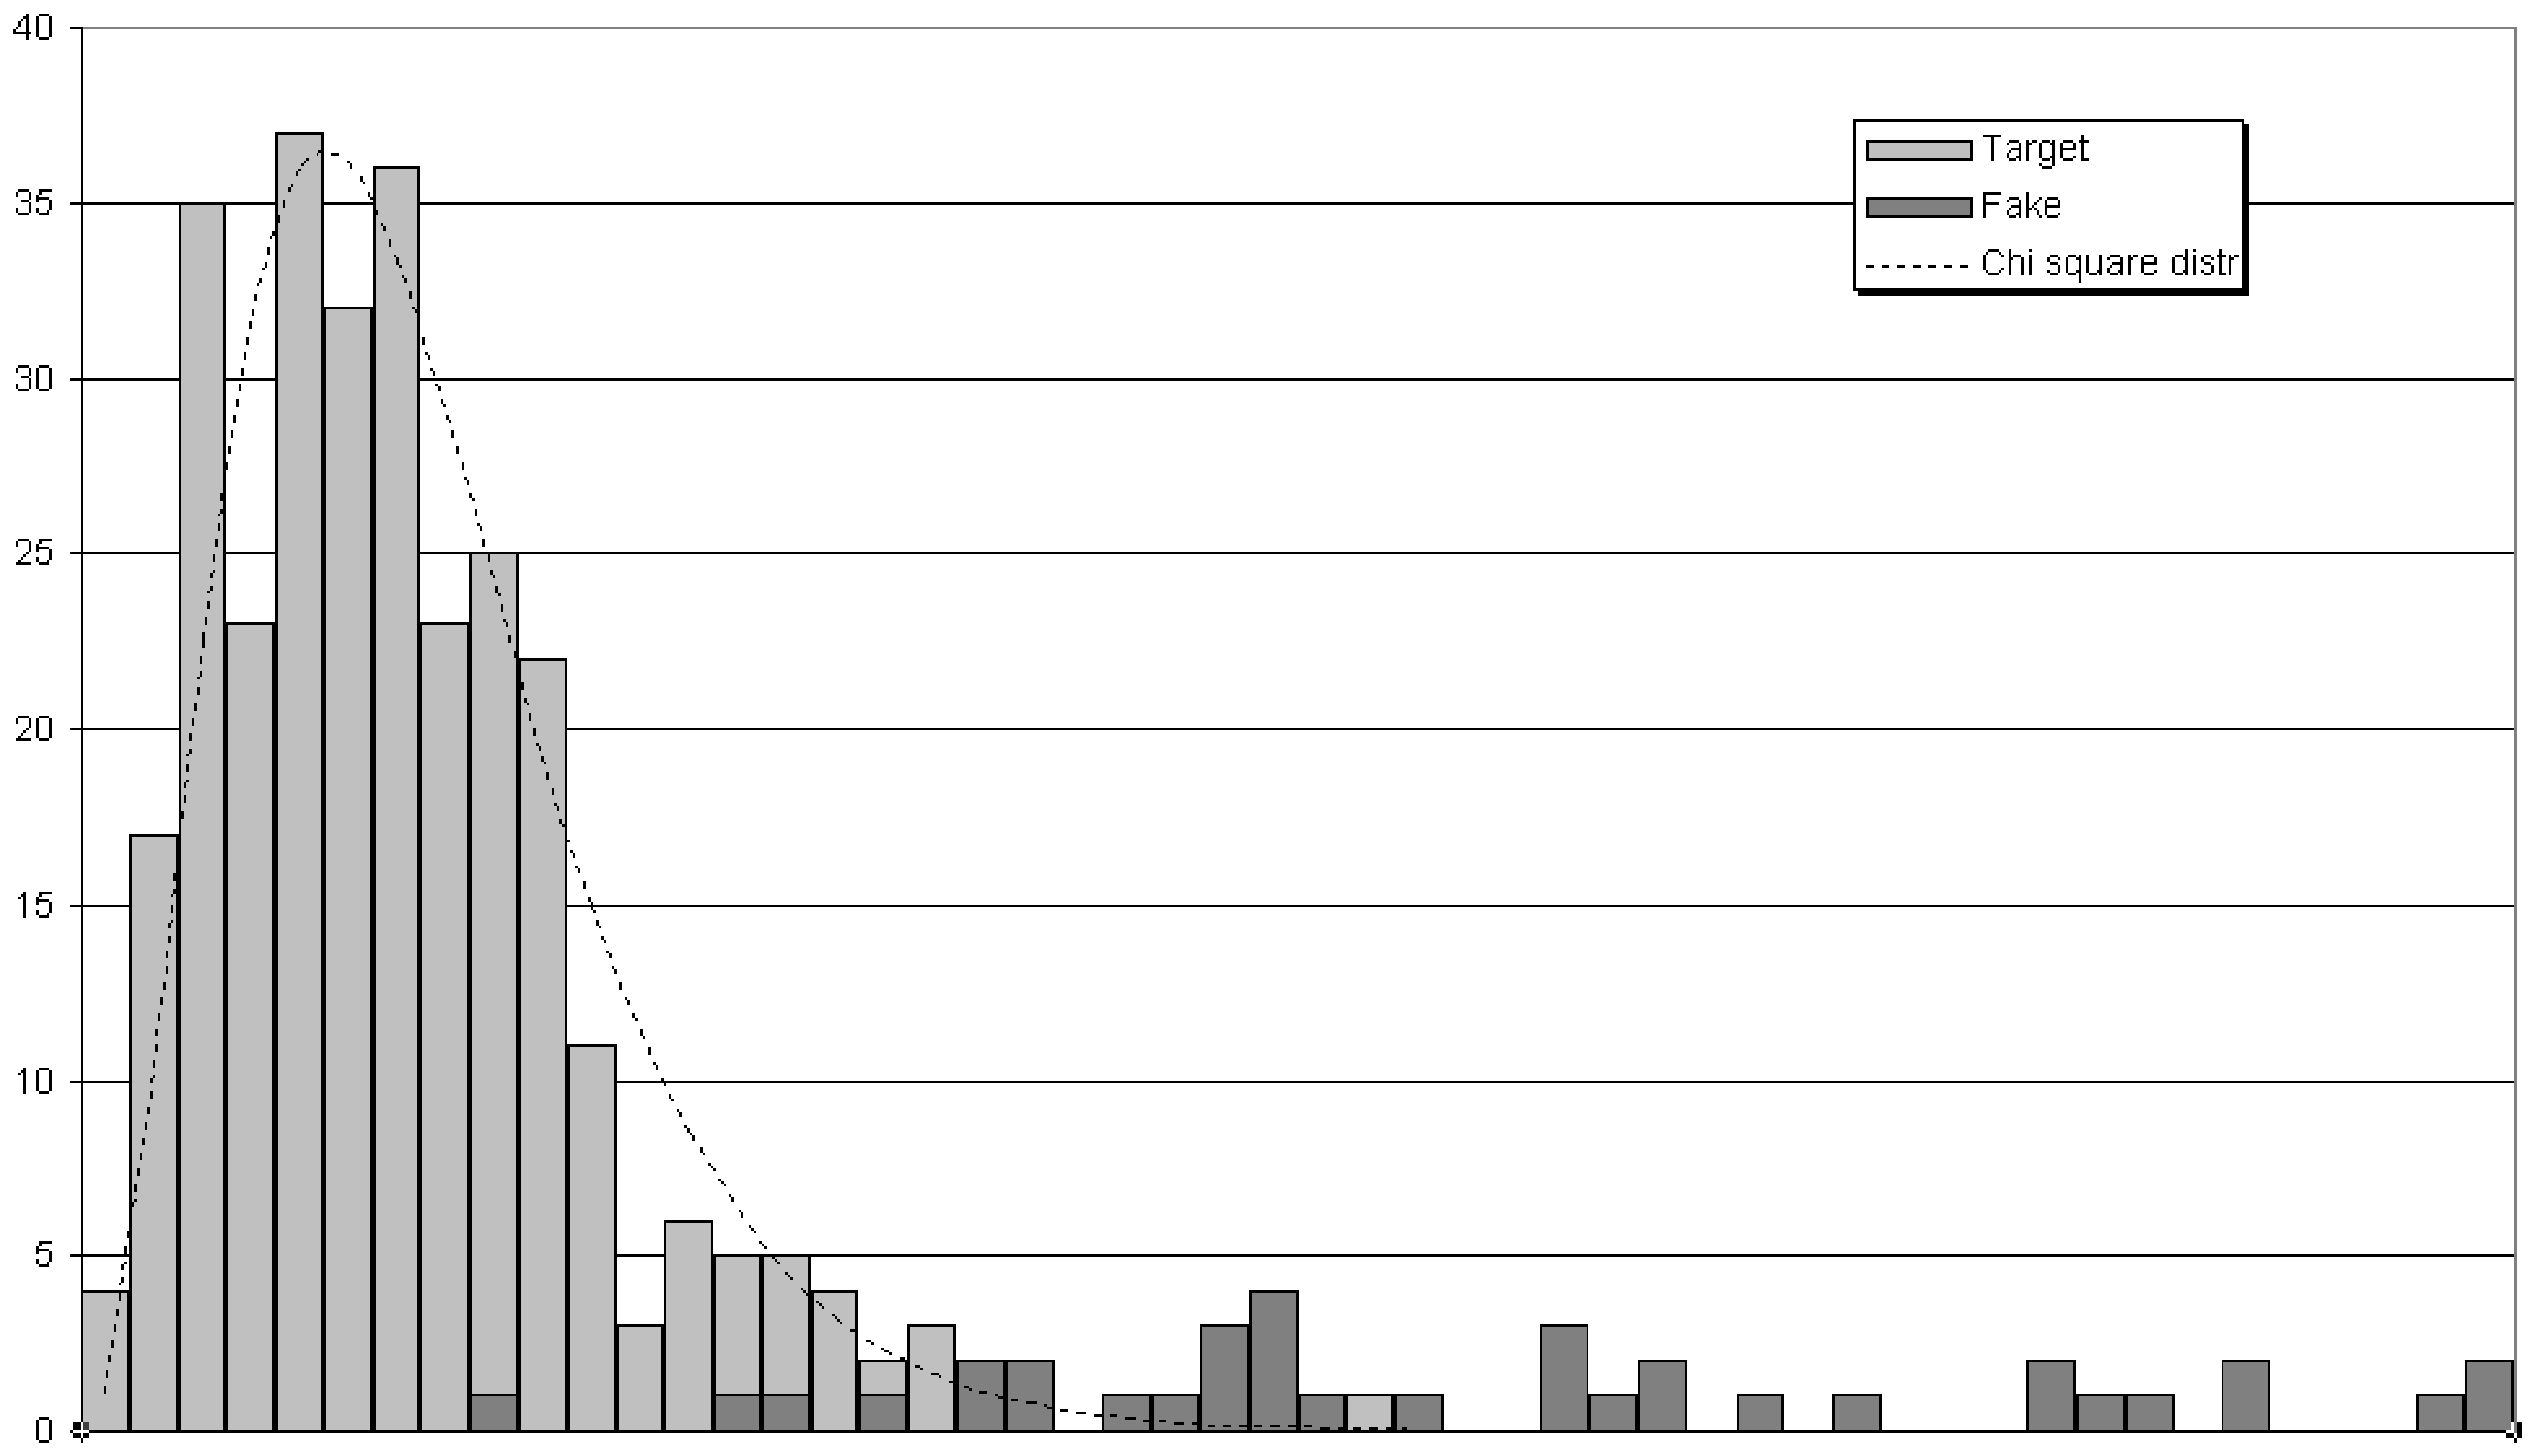
\includegraphics[width=12cm]{Figures/Mahalanobis}
\caption{Using the Mahalanobis distance to differentiate between
good and fake coins.}\label{fig:mahalanobis}
\end{figure}


Another field of application is the determination of cancer cells
from a biopsy. Parameters of cells --- size and darkness of
nucleus, granulation of the membrane --- can be measured
automatically and expressed in numbers. The covariance matrix can
be determined either using measurements of healthy cells or using
measurements of malignant cells. Identification of cancerous cells
can be automatized using the Mahalanobis distance.

\subsection{Mahalanobis distance --- General implementation}
\marginpar{Figure \ref{fig:dataminingclasses} with the box {\bf
MahalanobisCenter} grayed.} The final goal of the object
implementing the Mahalanobis distance is to compute the square
Mahalanobis distance as defined in equation \ref{eq:mahalanobis}.
This is achieved with the method {\tt distanceTo}. The inverse of
the covariance matrix as well as the average vector $\bar{\bf x}$
are contained within the object. We have called the object a
Mahalanobis center since it describes the {\sl center} of the
calibrating set.

To have a self-contained object, the Mahalanobis center is acting
as a \patstyle{facade} to the covariance accumulator of section
\ref{sec:covmatrix} for the accumulation of measurements. The
methods {\tt accumulate} and {\tt reset} are delegated to an
instance variable holding a covariance accumulator.

\noindent The Mahalanobis center has the following variables
\begin{description}
  \item[\tt accumulator] a covariance accumulator as described in section
\ref{sec:covmatrix};
  \item[\tt center] the vector $\bar{\bf x}$ and
  \item[\tt inverseCovariance] the inverse of the covariance
  matrix, that is $\inverse{V}$.
\end{description}
Our implementation is dictated by its future reuse in cluster
analysis (\cf section \ref{sec:mahalanobiscluster}). There, we
need to be able to accumulate measurements while using the result
of a preceding accumulation. Thus, computation of the center and
the inverse covariance matrix must be done explicitly with the
method {\tt computeParameters}.

There are two ways of creating a new instance. One is to specify
the dimension of the vectors which will be accumulated into the
object. The second supplies a vector as the tentative center. This
mode is explained in section \ref{sec:mahalanobiscluster}.

\subsection{Mahalanobis distance --- Smalltalk implementation}
Listing \ref{ls:mahalanobis} shows the implementation of a
Mahalanobis center in Smalltalk. The following code example shows
how to sort measurements using the Mahalanobis distance.
\begin{codeExample}
\begin{verbatim}

 | center calibrationServer dataServer data threshold|
 center := DhbMahalanobisCenter new: 5.
\end{verbatim}
\noindent{\tt<\sl The variable \tt calibrationServer \sl is setup
to read measurements from the calibrating set>}
\begin{verbatim}
 calibrationServer open.
 [ calibrationServer atEnd ]
      whileFalse: [ center accumulate: calibrationServer next ].
 calibrationServer close.
 center computeParameters.
\end{verbatim}
\noindent{\tt<\sl The variable \tt dataServer \sl is setup to read
the measurements to be sorted between accepted and rejected; the
variable \tt threshold \sl must also be determined or given\tt >}
\begin{verbatim}
 dataServer open.
 [ dataServer atEnd ]
      whileFalse: [ data := dataServer next.
                    ( center distanceTo: data) > threshold
                        ifTrue: [ self reject: data ]
                        ifFalse:[ self accept: data ].
                  ].
 dataServer close.
\end{verbatim}
\end{codeExample}
The first line after the declaration creates a new instance of a
Mahalanobis center for vectors of dimension 5. After setting up
the server for the calibrating set data from the calibrating set
are accumulated into the Mahalanobis center. At the end the
parameters of the Mahalanobis center are computed. Then, the
server for the other measurements is set up. The loop calculates
the distance to the Mahalanobis center for each measurements. Our
example supposes that the object executing this code has
implemented two methods {\tt accept} and {\tt reject} to process
accepted and rejected data.

\begin{listing} Smalltalk Mahalanobis center  \label{ls:mahalanobis}
$$\halign{ #\hfil&\quad#\hfil\cr {\sl Class}& {\Large\bf DhbMahalanobisCenter}\cr
{\sl Subclass of }&{\tt Object}\cr\noalign{\vskip 1ex}

{\sl Instance variable names:}&\parbox[t]{4 in}{\tt  center inverseCovariance accumulator }\cr\noalign{\vskip 1ex}}$$


Class methods
{\parskip 1ex\par\noindent}
{\bf new:} {\tt anInteger}
\begin{verbatim}
    ^ self new initialize: anInteger
\end{verbatim}
{\bf onVector:} {\tt aVector}
\begin{verbatim}
    ^ self new center: aVector
\end{verbatim}


Instance methods
{\parskip 1ex\par\noindent}
{\bf accumulate:} {\tt aVector}
\begin{verbatim}
    accumulator accumulate: aVector.
\end{verbatim}
{\bf center:} {\tt aVector}
\begin{verbatim}
    accumulator := DhbCovarianceAccumulator new: aVector size.
    center := aVector.
    inverseCovariance := DhbSymmetricMatrix identity: aVector size.
    ^ self
\end{verbatim}
{\bf computeParameters}
\begin{verbatim}
    center := accumulator average copy.
    inverseCovariance := accumulator covarianceMatrix inverse.
\end{verbatim}
{\bf count}
\begin{verbatim}
    ^ accumulator count
\end{verbatim}
{\bf distanceTo:} {\tt aVector}
\begin{verbatim}
    | delta |
    delta := aVector - center.
    ^ delta * inverseCovariance * delta
\end{verbatim}
{\bf initialize:} {\tt anInteger}
\begin{verbatim}
    accumulator := DhbCovarianceAccumulator new: anInteger.
    ^ self
\end{verbatim}
{\bf printOn:} {\tt aStream}
\begin{verbatim}
    accumulator count printOn: aStream.
    aStream nextPutAll: ': '.
    center printOn: aStream.
\end{verbatim}
{\bf reset}
\begin{verbatim}
    accumulator reset.
\end{verbatim}


\end{listing}



\section{Cluster analysis}
\label{sec:cluster} Cluster analysis --- also known as $K$-cluster
--- is a method to identify similarities between data. If the
dimension of the data is less than or equal than 3, graphical data
representation provides an easy way to identify data points having
some similarity. For more than 3 measurements, the human brain is
unable to clearly identify clustering.

Cluster analysis have been used successfully by the US army to
define a new classification of uniform sizes and in banks
\cite{BerLin}. British Telecom has used cluster analysis to detect
a phone fraud of large scale in the early 90's\footnote{Private
communication to the author.}.

\noindent The $K$-cluster algorithm goes as follows \cite{BerLin}:
\begin{enumerate}
  \item Pick up a set of centers where possible clusters may
  exist;
  \item place each data point into a cluster corresponding to the
  nearest center;
  \item when all data points have been processed, compute the
  center of each cluster;
  \item if the centers have changed, go back to point 2.
\end{enumerate}
This algorithm nicely maps itself to the framework of successive
approximations discussed in section \ref{sec:iteration}. We now
will investigate the steps of the algorithm in details.

\rubrique{Algorithm details} Picking up a set of centers
corresponds to the box labeled {\sl Compute or choose initial
object} of figure \ref{fig:iterfine}. Since one is looking for
unknown structure in the data there is little chance to make a
good guess on the starting values. The most general approach is to
pick up a few points at random from the existing data points to be
the initial cluster's centers.

The next two steps correspond to the box labeled {\sl Compute next
object} of figure \ref{fig:iterfine}. Here lies the gist of the
$K$-cluster algorithm. For each data point one first finds the
cluster whose center is the nearest to the data point. What is the
meaning of near? It depends on the problem. Let us just say at
this point that one needs to have a way of expressing the distance
between two data points. For the algorithm to converge the
distance must be a distance in the geometrical sense of the term.
In geometry, a distance is a numerical function of two vectors,
$d\left({\bf x},{\bf y}\right)$. For all vectors ${\bf x}$, ${\bf
y}$ and ${\bf z}$ the following conditions must be met by the
function
\begin{equation}
\nonumber
\begin{array}{l}
 d\left({\bf x},{\bf y}\right) \geq 0, \\
 d\left({\bf x},{\bf y}\right) = d\left({\bf y},{\bf x}\right), \\
 d\left({\bf x},{\bf y}\right) \leq d\left({\bf x},{\bf z}\right)
 + d\left({\bf z},{\bf y}\right).
\end{array}
\end{equation}
Furthermore, $d\left({\bf x},{\bf y}\right)=0$ if and only if
${\bf x}={\bf y}$. The simplest known distance function is the
Euclidean distance expressed as
\begin{equation}
\label{eq:eucliddist}
 d_E\left({\bf x},{\bf y}\right) = \sqrt{\left({\bf x}-{\bf y}\right)\cdot\left({\bf x}-{\bf
 y}\right)}.
\end{equation}
The square root in equation \ref{eq:eucliddist} is required for
the distance function to behave linearly on a one dimensional
subspace. The Euclidean distance corresponds to the notion of
distance in everyday life. In assessing the proximity of two
points, the square root is not needed.

After all points have been processed and assigned to a cluster,
the center of each cluster is obtained by taking the vector
average of all data points belonging to that cluster.

Then, one needs to determine whether the clusters have changed
since the last iteration. In the case of the $K$-cluster algorithm
it is sufficient to count the number of data points changing
clusters at each iteration. When the same data point are assigned
to the same clusters at the end of an iteration, the algorithm is
completed. The {\sl precision} used to stop the iterative process
is an integer in this case.

Figure \ref{fig:clustersteps} shows how the algorithm works for a
2-dimensional case.
\begin{figure}
\centering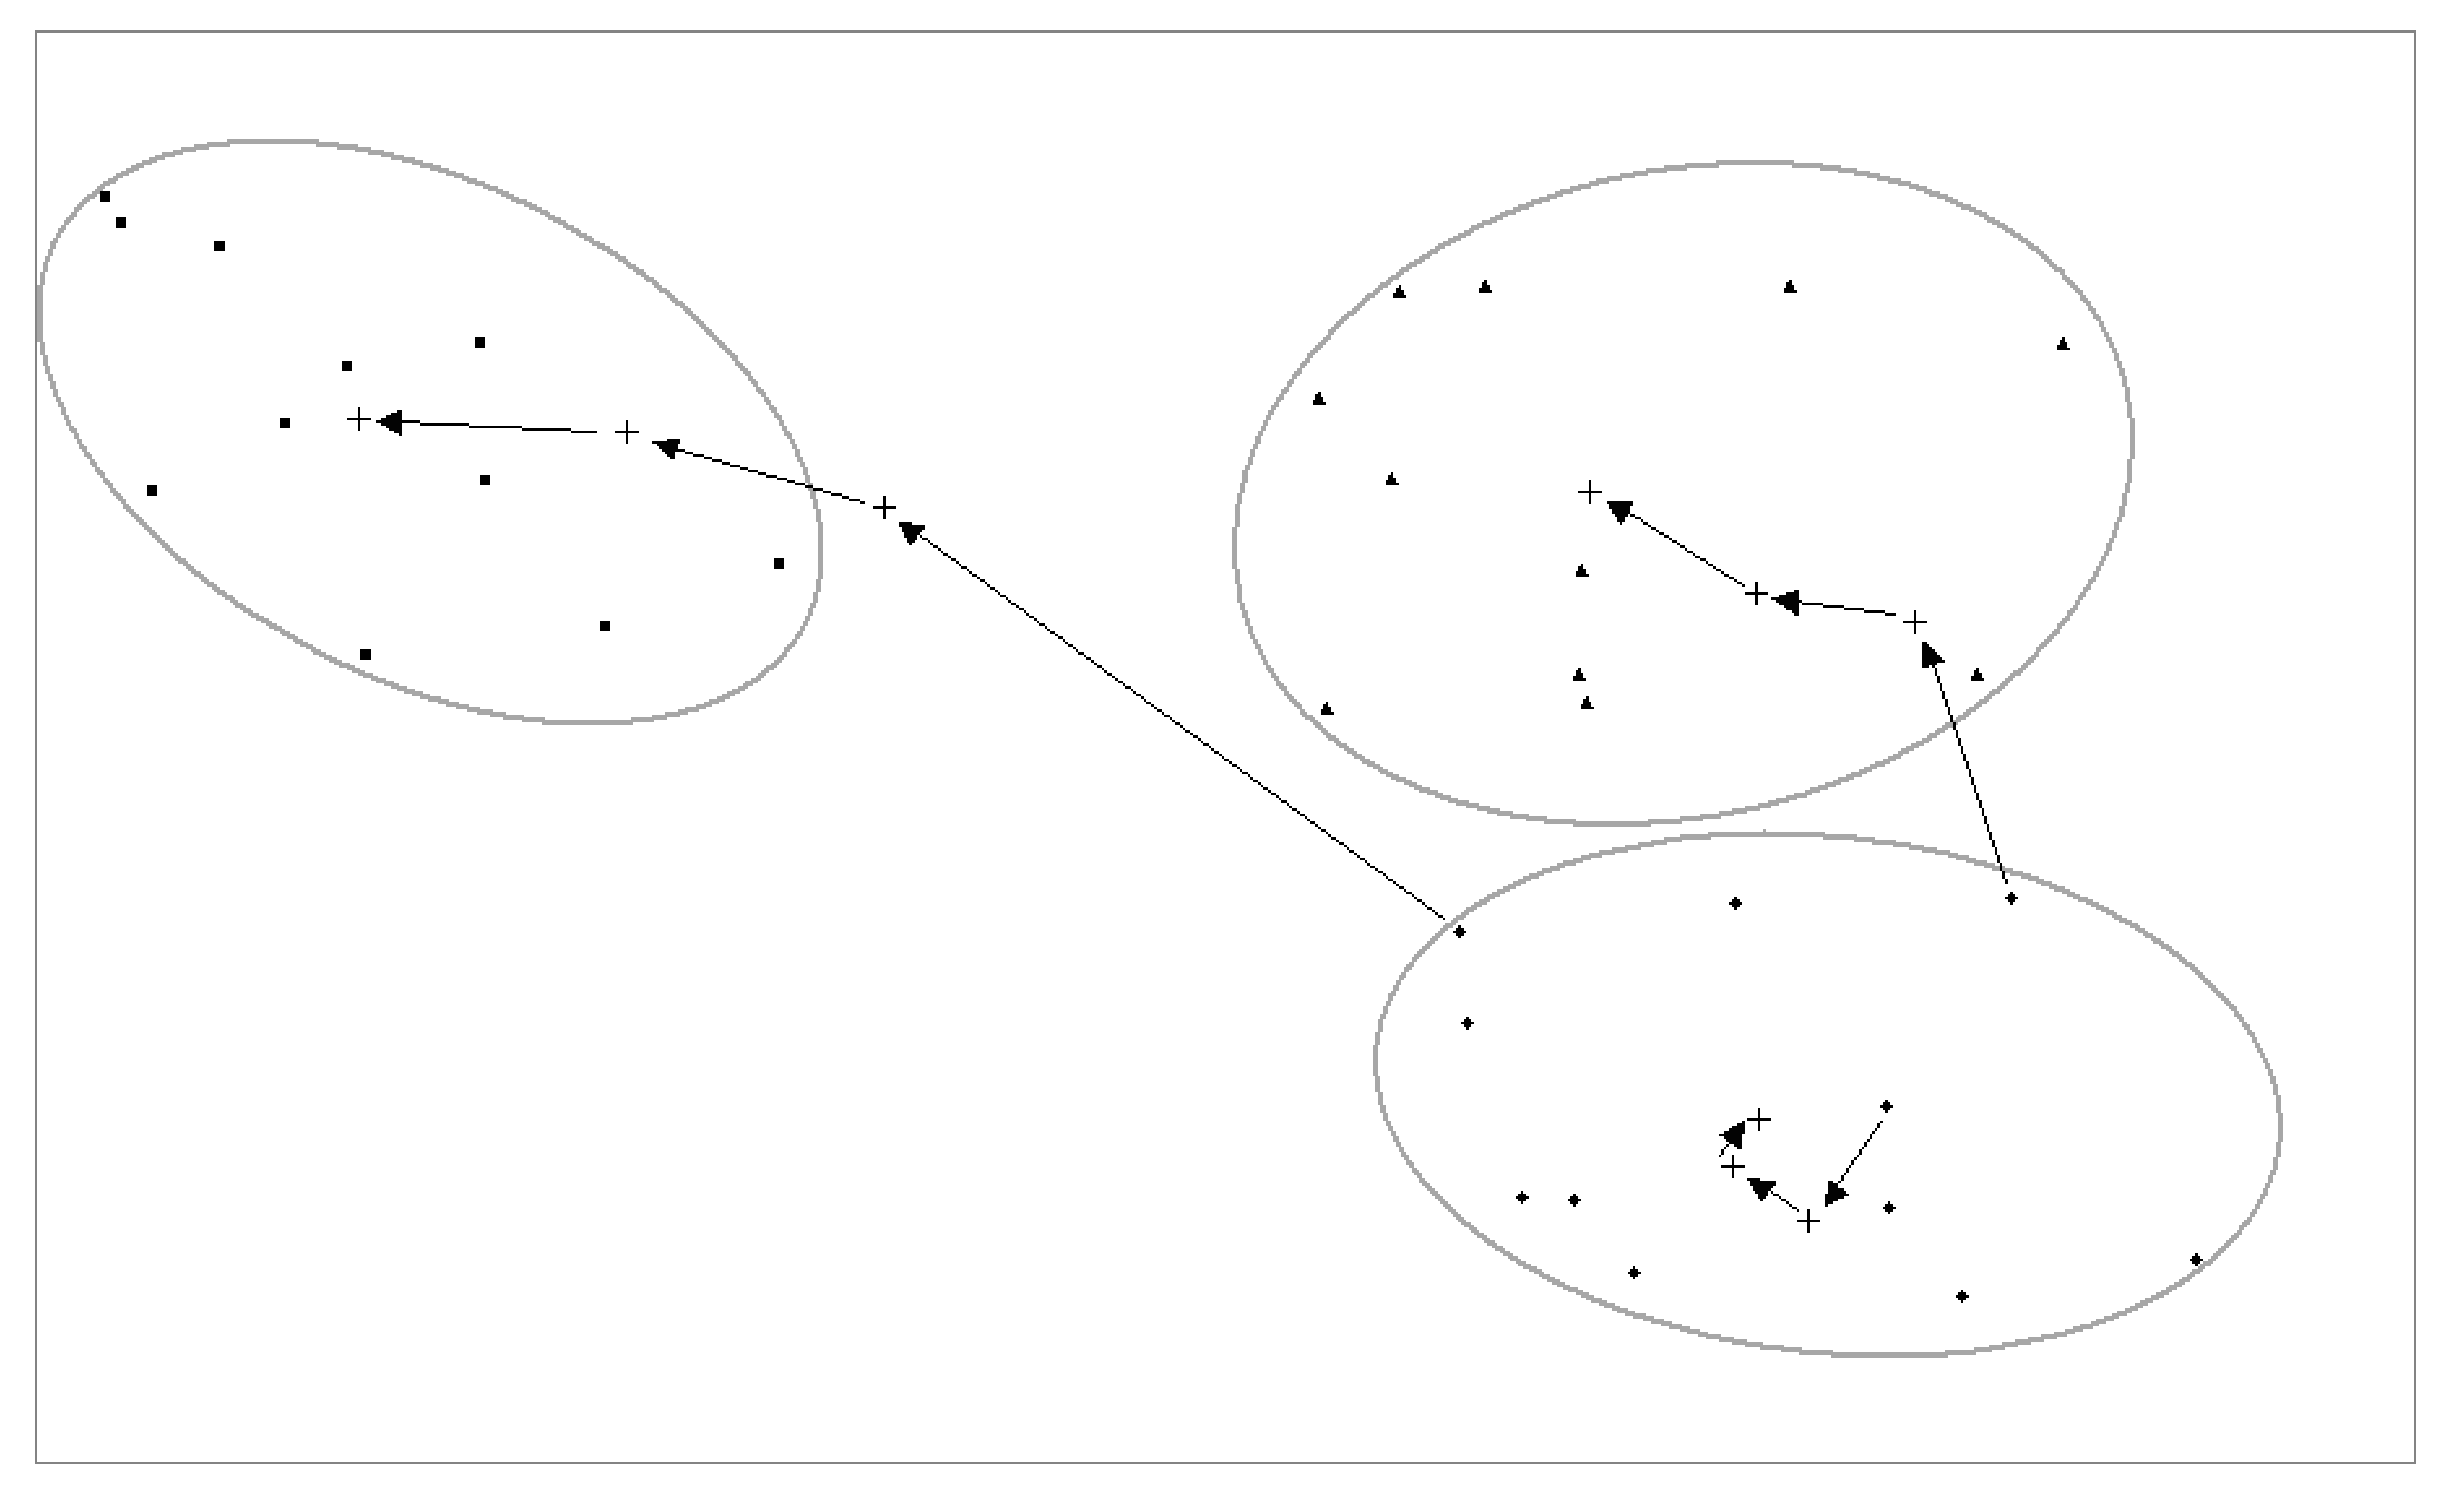
\includegraphics[width=11cm]{Figures/Clusters}
\caption{Example of cluster algorithm}\label{fig:clustersteps}
\end{figure}
Data points were generated randomly centered around 3 separated
clusters. Three random points were selected as starting points: in
this example the random choice was particularly unlucky since the
three starting points all belong to the same cluster.
Nevertheless, convergence was attained after 5
iterations\footnote{The last iteration is not visible since the
centers did not change.}.

\rubrique{Fine points} This simple example is admittedly not
representative. However, this is not because of the small
dimension nor because of the well separated clusters. It is
because we knew in advance the number of clusters, 3 in this case.
If we had started with 5 initial clusters, we would have ended up
with 5 clusters, according to the expression, {\sl garbage in,
garbage out}, well-known among programmers.

One can modify the original algorithm to prune insignificant
clusters from the search. This additional step must be added
between steps 2 and 3. How to characterize an insignificant
cluster? This often depends on the problem at hand. One thing for
sure is that clusters with 0 elements should be left out. Thus,
one easy method to prune insignificant clusters is to place a
limit of the number of data points contained in each cluster. That
limit should not be too high, however, otherwise most clusters
will never get a chance of accumulating a significant amount of
data points during the first few iterations.

\subsection{Cluster analysis --- General implementation}
\marginpar{Figure \ref{fig:dataminingclasses} with the boxes {\bf
ClusterFinder} and {\bf Cluster} grayed.} Our implementation of
the $K$-cluster algorithm uses two classes: {\tt ClusterFinder}
and {\tt Cluster}.

The class {\tt Cluster} describes the behavior of a cluster. It is
an abstract class. Subclasses implements the various strategies
needed by the algorithm: distance calculation and pruning of
insignificant clusters. The abstract class has only one instance
variable, {\tt previousSampleSize}, keeping the count of data
points accumulated in the previous iteration. A cluster must be
able to return the number of data points contained in the cluster.
The method {\tt changes} gives the number of data points which
have changed cluster since the last iteration. The method {\tt
isInsignificantIn} determines whether a cluster must be pruned
from the process. The method {\tt isUndefined} allows the
identification of clusters whose centers have not yet been
defined. This method is used by the cluster finder to initialize
undefined clusters with the data points before starting the
iterative process.

An instance of a subclass of {\tt cluster} must implement the
following methods to interact with the class {\tt ClusterFinder}:
\begin{description}
  \item[\tt distanceTo] the argument of this method is a vector
  representing the data point; the returned value is the distance
  between the supplied vector and the center of the cluster; any
  subclass of {\tt Cluster} can implement a suitable distance function
  as well as its own representation of the center;
  \item[\tt accumulate] the argument of this method is a vector
  representing the data point; this method is called when the
  cluster finder has determined that the data point must be placed
  within this cluster;
  \item[\tt changes] this method returns the number of data points
  which have been added to and removed from the cluster since the
  last iteration; the default implementation only calculates the
  difference between the number currently in the cluster and the
  number in the previous iteration; this simple approach works in
  practice\footnote{Of course, one can construct cases where this
  simple approach fails. Such cases, however, correspond to
  situations where data points are oscillating between clusters
  and, therefore, do not converge. I have never met such cases in practice.};
  \item[\tt sampleSize] this method returns the number of data
  points actually accumulated into the cluster;
  \item[\tt reset] this method calculates the position of the new
  center at the end of an iteration; the default implementation
  stores the size of the previous sample.
\end{description}

\note{A reader knowledgeable in patterns will think of using a
\patstyle{Strategy} pattern to implement the distance. I have
tried this approach, but the resulting classes were much more
complex for little gain. It is easier to implement subclasses of
{\tt Cluster}. Each subclass can not only implement the distance
function, but can also choose how to accumulate data points:
accumulation or storage.}

The concrete class {\tt EuclideanCluster} calculates the square of
the Euclidean distance as defined in equation \ref{eq:eucliddist}.
Using Euclidean distance requires that the components of the data
vector have comparable scales. Cluster analysis with Euclidean
clusters requires data preparation in general.

The class {\tt ClusterFinder} implements the algorithm itself.
This class is a subclass of the class for iterative processes
described in section \ref{sec:iteration}. The result of the
iterative process is an array of clusters. The class {\tt
ClusterFinder}  needs the following instance variables:
\begin{description}
  \item[\tt dataServer] a data server object as described in
  section \ref{sec:dataserver}; this object is used to iterate on
  the data points;
  \item[\tt dataSetSize] a counter to keep track of the number of
  data points; this instance variable is combined with the next to
  provide a first order pruning strategy;
  \item[\tt minimumRelativeClusterSize] the minimum relative size
  of a significant cluster; the minimum cluster
  size is computed at each iteration by taking the product of this variable with the
  variable {\tt dataSetSize}.
\end{description}

The class {\tt ClusterFinder} uses an instance of the data server
to iterate over the data points. before starting the search the
client application can assign the list of initial clusters (step 1
of the algorithm . By default, the minimum relative size of the
cluster is set to 0. A convenience method allows creating
instances for a given data server and an initial set of clusters.

The method {\tt initializeIterations} scans all clusters and looks
for undefined clusters. The center of each undefined cluster is
assigned to a data point read from the data server. This assumes
that the data points have been collected randomly.

\noindent The method {\tt evaluateIteration} processes each data
point: first, it finds the index of the cluster nearest to the
data point; then, the data point is accumulated into that cluster.
After processing the data points, the clusters are processed to
compute the new position of their centers and insignificant
clusters are removed from the search. These tasks are performed
within a method named {\tt collectChangesAndResetClusters}. This
method returns the number of data points which have changed
cluster. The determination whether or not a cluster is significant
is delegated to each cluster with the method {\tt
isInsignificant}. Thus, any subclass of cluster can implement its
own strategy. The argument of the method {\tt isInsignificant} is
the cluster finder to provide each cluster with global information
if needed.

\noindent The method {\tt finalizeIterations} just closes the data
server.

\subsection{Cluster analysis --- Smalltalk implementation}
Listing \ref{ls:clusterfinder} shows the implementation of the
$K$-cluster algorithm in Smalltalk. The following code example
shows how to implement a search for clusters.
\begin{codeExample}
\begin{verbatim}

 | dataServer finder clusters |
\end{verbatim}
\noindent{\tt<\sl The variable \tt dataServer \sl is setup to read
measurements from the calibrating set>}
\begin{verbatim}
 finder := DhbClusterFinder new: 5 server: dataServer
\end{verbatim}
\hfil{\tt type: <\sl a concrete subclass of \tt Cluster>.}
\begin{verbatim}
 finder minimumRelativeClusterSize: 0.1.
 clusters := finder evaluate.
\end{verbatim}
\end{codeExample}
After setting up a data server to read the data point, an instance
of class {\tt DhbClusterFinder} is created. the number of desired
clusters is set to 5. The class of the clusters is specified. The
next line sets the minimum relative size of each cluster to be
kept during the iteration. Finally, the $K$-cluster algorithm is
performed and clusters are retrieved from the finder object.

The abstract class {\tt DhbCluster} is implemented with an
instance variable {\tt accumulator}. The cluster delegates the
responsibility of accumulating the data points to this variable.
It is assumed that the object in {\tt accumulator} implements the
interface defined by the vector accumulators described in section
\ref{sec:scovmatrix}.

The class {\tt DhbClusterFinder} can be created in two ways. An
application can set the list of initial clusters and the data
server using the methods {\tt cluster} and {\tt dataServer}
respectively. The convenience class creation method {\tt
new:server:type:} allows to specify the initial number of
clusters, the data server and the class of the clusters. When this
method is used, the collection of clusters is created when the
instance of {\tt DhbClusterFinder} is initialized; each cluster is
created in an undefined state.

\begin{listing} Smalltalk $K$-cluster algorithm \label{ls:clusterfinder}
$$\halign{ #\hfil&\quad#\hfil\cr {\sl Class}& {\Large\bf DhbCluster}\cr
{\sl Subclass of }&{\tt Object}\cr\noalign{\vskip 1ex}

{\sl Instance variable names:}&\parbox[t]{4 in}{\tt  accumulator previousSampleSize }\cr\noalign{\vskip 1ex}}$$

Instance methods
{\parskip 1ex\par\noindent}
{\bf accumulate:} {\tt aVector}
\begin{verbatim}
    accumulator accumulate: aVector.
\end{verbatim}
{\bf centerOn:} {\tt aVector}
\begin{verbatim}
    self subclassResponsibility
\end{verbatim}
{\bf changes}
\begin{verbatim}
    ^ (self sampleSize - previousSampleSize) abs
\end{verbatim}
{\bf distanceTo:} {\tt aVector}
\begin{verbatim}
    ^ self subclassResponsibility
\end{verbatim}
{\bf initialize}
\begin{verbatim}
    previousSampleSize := 0.
    ^ self
\end{verbatim}
{\bf isInsignificantIn:} {\tt aClusterFinder}
\begin{verbatim}
    ^ self sampleSize <= aClusterFinder minimumClusterSize
\end{verbatim}
{\bf isUndefined}
\begin{verbatim}
    ^ self subclassResponsibility
\end{verbatim}
{\bf reset}
\begin{verbatim}
    previousSampleSize := self sampleSize.
    self collectAccumulatorResults.
    accumulator reset
\end{verbatim}
{\bf sampleSize}
\begin{verbatim}
    ^ accumulator count
\end{verbatim}


$$\halign{ #\hfil&\quad#\hfil\cr {\sl Class}& {\Large\bf DhbClusterFinder}\cr
{\sl Subclass of }&{\tt DhbIterativeProcess}\cr\noalign{\vskip 1ex}

{\sl Instance variable names:}&\parbox[t]{4 in}{\tt  dataServer dataSetSize minimumRelativeClusterSize }\cr\noalign{\vskip 1ex}}$$


Class methods
{\parskip 1ex\par\noindent}
{\bf new:} {\tt anInteger} {\bf server:} {\tt aClusterDataServer} {\bf type:} {\tt aClusterClass}
\begin{verbatim}
    ^ super new initialize: anInteger server: aClusterDataServer type: 
                                                         aClusterClass
\end{verbatim}



Instance methods
{\parskip 1ex\par\noindent}
{\bf accumulate:} {\tt aVector}
\begin{verbatim}
    ( result at: ( self indexOfNearestCluster: aVector)) accumulate: 
                                                              aVector.
\end{verbatim}
{\bf clusters:} {\tt aCollectionOfClusters}
\begin{verbatim}
    result := aCollectionOfClusters.
\end{verbatim}
{\bf collectChangesAndResetClusters}
\begin{verbatim}
    | hasEmptyClusters changes |
    changes := 0.
    hasEmptyClusters := false.
    result do: 
            [ :each | 
            changes := each changes + changes.
            ( each isInsignificantIn: self)
                ifTrue: 
                    [each centerOn: nil.
                    hasEmptyClusters := true]
                ifFalse: [each reset].
            ].
    hasEmptyClusters 
        ifTrue: [result := result reject: [:each | each 
                                                        isUndefined]].
    ^ changes / 2
\end{verbatim}
{\bf dataServer:} {\tt aClusterDataServer}
\begin{verbatim}
    dataServer := aClusterDataServer.
\end{verbatim}
{\bf evaluateIteration}
\begin{verbatim}
    dataServer reset.
    dataSetSize := 0.
    [ dataServer atEnd]
        whileFalse:[ self accumulate: dataServer next.
                     dataSetSize := dataSetSize + 1.
                    ].
    ^ self collectChangesAndResetClusters
\end{verbatim}
{\bf finalizeIterations}
\begin{verbatim}
    dataServer close
\end{verbatim}
{\bf indexOfNearestCluster:} {\tt aVector}
\begin{verbatim}
    | distance index |
    index := 1.
    distance := ( result at: 1) distanceTo: aVector.
    2 to: result size do:
        [ :n | | x |
          x := ( result at: n) distanceTo: aVector.
          x < distance
            ifTrue: [ distance := x.
                      index := n.
                    ].
        ].
    ^ index
\end{verbatim}
{\bf initialize:} {\tt anInteger} {\bf server:} {\tt aClusterDataServer} {\bf type:} {\tt aClusterClass}
\begin{verbatim}
    self dataServer: aClusterDataServer.
    self clusters: ( (1 to: anInteger) collect: [ :n | aClusterClass 
                                                                new]).
    minimumRelativeClusterSize := 0.
    ^ self
\end{verbatim}
{\bf initializeIterations}
\begin{verbatim}
    dataServer open.
    result 
        do: [:each | each isUndefined ifTrue: [each centerOn: 
                                                     dataServer next]]
\end{verbatim}
{\bf minimumClusterSize}
\begin{verbatim}
    ^ (minimumRelativeClusterSize * dataSetSize) rounded
\end{verbatim}
{\bf minimumRelativeClusterSize:} {\tt aNumber}
\begin{verbatim}
    minimumRelativeClusterSize := aNumber max: 0.
\end{verbatim}
{\bf printOn:} {\tt aStream}
\begin{verbatim}
    aStream nextPutAll: 'Iterations: '.
    iterations printOn: aStream.
    result do: [ :each | aStream cr. each printOn: aStream ].
\end{verbatim}

\end{listing}
Listing \ref{ls:euclidcluster} shows the implementation of the
concrete cluster class {\tt DhbEuclideanCluster}. The
corresponding accumulator is an instance of class {\tt
DhbVectorAccumulator}. Data points are directly accumulated into
the accumulaotr; individual data points are not kept.
\begin{listing} Smalltalk implementation of an Euclidean cluster \label{ls:euclidcluster}
$$\halign{ #\hfil&\quad#\hfil\cr {\sl Class}& {\Large\bf DhbEuclideanCluster}\cr
{\sl Subclass of }&{\tt DhbCluster}\cr\noalign{\vskip 1ex}

{\sl Instance variable names:}&\parbox[t]{4 in}{\tt  center }\cr\noalign{\vskip 1ex}}$$


Instance methods
{\parskip 1ex\par\noindent}
{\bf centerOn:} {\tt aVector}
\begin{verbatim}
    center := aVector.
    accumulator := DhbVectorAccumulator new: aVector size.

\end{verbatim}
{\bf collectAccumulatorResults}
\begin{verbatim}
    center := accumulator average copy.

\end{verbatim}
{\bf distanceTo:} {\tt aVector}
\begin{verbatim}
    ^( aVector - center) norm

\end{verbatim}
{\bf isUndefined}
\begin{verbatim}
    ^center isNil

\end{verbatim}
{\bf printOn:} {\tt aStream}
\begin{verbatim}
    accumulator count printOn: aStream.
    aStream nextPutAll: ': '.
    center printOn: aStream.

\end{verbatim}


\end{listing}


\section{Covariance clusters}
\label{sec:mahalanobiscluster} As we have seen in section
\ref{sec:mahalanobis} the Mahalanobis distance is a distance in
the geometrical sense. Thus, this distance can be used by the
$K$-cluster algorithm. We call clusters using the Mahalanobis
distance covariance clusters since the metric for the distance is
based on the covariance matrix.

The normalizing properties of the Mahalanobis distance makes it
ideal for this task. When Euclidean distance is used, the metric
remains the same in all directions. Thus, the extent of each
cluster has more or less circular shapes. With the Mahalanobis
distance the covariance metric is unique for each cluster. Thus,
covariance clusters can have different shapes since the metric
adapts itself to the shape of each cluster. As the algorithm
progresses the metric changes dynamically.

\subsection{Covariance clusters --- General implementation}
\marginpar{Figure \ref{fig:dataminingclasses} with the boxes {\bf
CovarianceCluster} grayed.} Covariance clusters need little
implementation. All tasks are delegated to a Mahalanobis center
described in section \ref{sec:mahalanobis}. Listing
\ref{ls:mahacluster} shows the Smalltalk implementation and the
Java implementation is shown in listing \ref{lj:mahacluster}.

\begin{listing} Smalltalk covariance cluster \label{ls:mahacluster}
$$\halign{ #\hfil&\quad#\hfil\cr {\sl Class}& {\Large\bf DhbCovarianceCluster}\cr
{\sl Subclass of }&{\tt DhbCluster}\cr\noalign{\vskip 1ex}

{\sl Instance variable names:}&\parbox[t]{4 in}{\tt  center }\cr\noalign{\vskip 1ex}}$$


Instance methods
{\parskip 1ex\par\noindent}
{\bf centerOn:} {\tt aVector}
\begin{verbatim}
    accumulator := aVector ifNotNil: [ :v | DhbMahalanobisCenter 
                                                         onVector: v].

\end{verbatim}
{\bf collectAccumulatorResults}
\begin{verbatim}
    accumulator computeParameters.

\end{verbatim}
{\bf distanceTo:} {\tt aVector}
\begin{verbatim}
    ^accumulator distanceTo: aVector

\end{verbatim}
{\bf isUndefined}
\begin{verbatim}
    ^accumulator isNil

\end{verbatim}
{\bf printOn:} {\tt aStream}
\begin{verbatim}
    accumulator printOn: aStream.

\end{verbatim}


\end{listing}


\ifx\wholebook\relax\else\end{document}\fi
